\chapter{Propuesta}
\begin{figure}[h]
  \label{figurapropuesta}
  \centering
  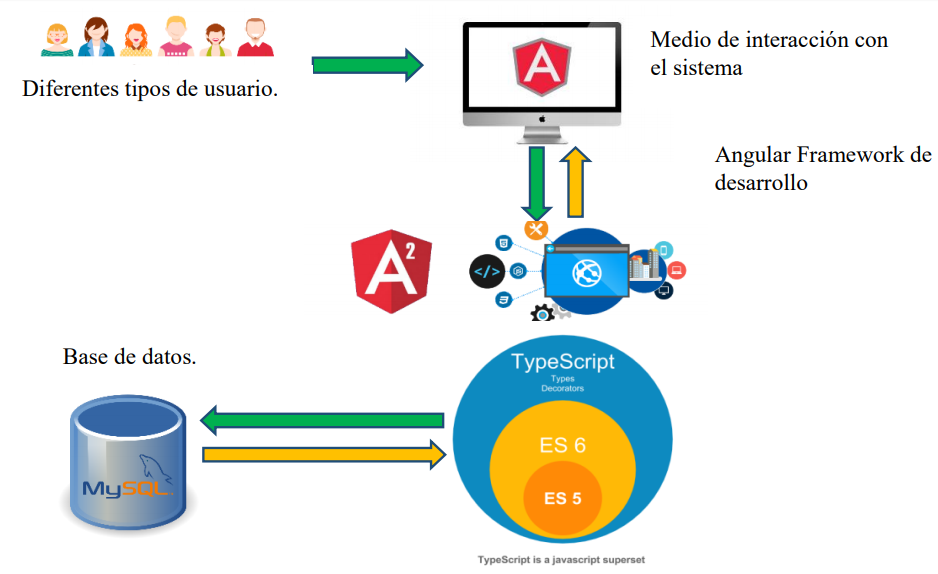
\includegraphics[scale=.5]{lib/assets/propuesta-tecnica}
  \caption{Propuesta técnica de proyecto.}
\end{figure}

\section{Angular }
Angular es un Framework desarrollado por los ingenieros de Google, el cual está basado en programación por componentes, los cuales son muy útiles ya que ayudan a reducir grandes cantidades de código reutilizando los componentes en todo el proyecto, pudiendo así tener un mejor control de proyectos de gran escalabilidad. El desarrollo de este sistema tendrá un gran reto que será justamente el control y seguridad de los datos de los pacientes, por ello se decidió utilizar Angular, el cual es un framework muy maduro y con una enorme comunidad que contribuye a su desarrollo. Cuenta con una documentación muy vasta, facilitando así un mejor y óptimo desarrollo, ahorrando tiempo, esfuerzo y además es fácil su despliegue en los servidores. \cite{Angular}

\section{Bulma}
Bulma un framework CSS basado en Flexbox. Una hoja de estilos con diseños predefinidos, basándose en las líneas de diseño propuestas por Google en Material Design.
Ocuparemos de Bulma en el proyecto para el desarrollo de las vistas que interactuaran con el usuario final, teniendo esta una interfaz más agradable y amigable, además como las líneas de diseño están predefinidas, nos ahorraremos mucho tiempo y su interacción con el framework es muy buena. \cite{Bulma}

\section{ Mysql}
Base de datos relacional de código abierto, el cual se trabaja con SQL (Structured Query Language).
El utilizar MySql en el proyecto se debe a que es uno de los mejores gestores con mejor rendimiento, los bajos requisitos para poder ejecutarse, la facilidad de configuración, gran compatibilidad con muchos sistemas operativos, además es uno de los más seguros y la interacción con Angular es fantástica. \cite{mysql}

\section{Typescript}
Es un superset de javascript el cual funciona muy bien con proyectos de gran tamaño, la característica principal del typescript es que reduce significativamente el tamaño del código y lo vuelve a este mucho más comprensible y es el lenguaje que Angular ha adoptado en su esquema de desarrollo.
\subsection{¿Qué es un superset?}

Se trata de un lenguaje escrito sobre otro lenguaje. En este caso Typescript es eso, un lenguaje basado en el original, ofreciéndonos grandes beneficios como el descrito anteriormente, aunque existen otros beneficios. Por ejemplo, mientras otros superset de JavaScript nos alejan del código original, Typescript, por el contrario, es muy similar a Javascript y a C# gracias a que su creador posee conocimientos de ambos lenguajes \cite{typeScript}
